%=============================================================================
%  MIVA-KNIGHT: Full Pipeline Technical & Layman Documentation
%  Author: Kayode (Oluwakayode) Soyinka  |  IT 581 — Capstone, Month 4
%  Supervisor: Dr. Baidya Saha  |  Concordia University of Edmonton
%=============================================================================
\documentclass[12pt, a4paper]{article}

%--- Encoding & fonts ---------------------------------------------------------
\usepackage[T1]{fontenc}
\usepackage[utf8]{inputenc}


%--- Maths --------------------------------------------------------------------
\usepackage{amsmath, amssymb, amsthm, mathtools}

%--- Algorithms ---------------------------------------------------------------
\usepackage{algorithm}
\usepackage{algpseudocode}

%--- TikZ / Figures -----------------------------------------------------------
\usepackage{tikz}
\usetikzlibrary{
  shapes.geometric, arrows.meta, positioning,
  fit, backgrounds, calc, patterns, decorations.pathreplacing,
  shadows, matrix, chains
}

%--- Layout -------------------------------------------------------------------
\usepackage[margin=2.5cm]{geometry}
\usepackage{setspace}
\onehalfspacing
\usepackage{parskip}

%--- Colours ------------------------------------------------------------------
\usepackage{xcolor}
\definecolor{frozenblue}{RGB}{180,210,240}
\definecolor{trainableorange}{RGB}{255,210,160}
\definecolor{medicalgreen}{RGB}{180,230,200}
\definecolor{generalyellow}{RGB}{255,245,180}
\definecolor{darknavy}{RGB}{30,50,90}
\definecolor{midgray}{RGB}{100,100,100}
\definecolor{lightgray}{RGB}{235,235,235}
\definecolor{cocoviolet}{RGB}{220,195,240}
\definecolor{rococyan}{RGB}{180,230,245}
\definecolor{infonce}{RGB}{255,225,210}
\definecolor{pmicolor}{RGB}{210,240,210}
\definecolor{faisscolor}{RGB}{210,230,255}

%--- Tables -------------------------------------------------------------------
\usepackage{booktabs, array, longtable, multirow}
\usepackage{colortbl}

%--- Lists --------------------------------------------------------------------
\usepackage{enumitem}

%--- Captions & hyperlinks ----------------------------------------------------
\usepackage{caption}
\usepackage[hidelinks, colorlinks=false]{hyperref}

%--- Theorem environments -----------------------------------------------------
\theoremstyle{definition}
\newtheorem{definition}{Definition}[section]
\newtheorem{axiom}{Axiom}[section]

\theoremstyle{plain}
\newtheorem{theorem}{Theorem}[section]
\newtheorem{lemma}[theorem]{Lemma}
\newtheorem{corollary}[theorem]{Corollary}
\newtheorem{proposition}[theorem]{Proposition}

\theoremstyle{remark}
\newtheorem{remark}{Remark}[section]
\newtheorem{example}{Example}[section]

%--- Custom commands ----------------------------------------------------------
\newcommand{\R}{\mathbb{R}}
\newcommand{\Sphere}{\mathbb{S}}
\newcommand{\norm}[1]{\left\|#1\right\|_2}
\newcommand{\dotprod}[2]{\langle #1,\, #2 \rangle}
\newcommand{\KG}{\mathcal{G}}
\newcommand{\Emb}{\mathcal{E}}
\newcommand{\layman}[1]{%
  \vspace{4pt}%
  \noindent\colorbox{lightgray}{\parbox{\dimexpr\linewidth-2\fboxsep}{%
    \textbf{\textit{In plain terms:}} #1}}%
  \vspace{4pt}%
}

%=============================================================================
\begin{document}

%--- Title page ---------------------------------------------------------------
\begin{titlepage}
  \centering
  \vspace*{2cm}
  {\Huge\bfseries MIVA-KNIGHT}\\[0.5em]
  {\Large Multimodal Interactive Voice Assistant\\
   with Knowledge-driven Hybrid Intelligence\\
   and Adaptive Domain Transfer}\\[2em]
  \rule{\linewidth}{1pt}\\[1em]
  {\large\bfseries Full Pipeline Technical Reference}\\
  {\large Algorithms $\cdot$ Theorems $\cdot$ Lemmas $\cdot$ Axioms}\\[2em]
  \rule{\linewidth}{0.5pt}\\[1em]
  \begin{tabular}{rl}
    \textbf{Student:}    & Kayode (Oluwakayode) Soyinka \\
    \textbf{Course:}     & IT 581 --- Capstone Project \\
    \textbf{Supervisor:} & Dr.\ Baidya Saha \\
    \textbf{Institution:}& Concordia University of Edmonton \\
    \textbf{Month:}      & 4 --- Medical Domain Transfer \\
  \end{tabular}\\[3em]
  \tableofcontents
\end{titlepage}

%=============================================================================
\newpage
\section{Project Overview and Core Thesis Claim}
\label{sec:overview}

\subsection{What Is MIVA-KNIGHT?}

MIVA-KNIGHT (\textbf{M}ultimodal \textbf{I}nteractive \textbf{V}oice \textbf{A}ssistant with \textbf{K}nowledge-driven \textbf{H}ybrid \textbf{I}ntelligence and Adaptive Domain Transfer) is a research prototype that can answer spoken questions using three types of input: \emph{text}, \emph{images}, and \emph{voice}. Rather than relying on a single large language model, it combines specialised encoder networks, a fast vector index, a semantically-enriched knowledge graph, and a lightweight language model to generate grounded, verifiable answers.

\layman{Think of MIVA-KNIGHT as a multi-sense research assistant. A human expert uses eyes (images), ears (voice), and reading (text) simultaneously. MIVA-KNIGHT does the same electronically: it listens to a spoken question, looks at any attached image, reads related documents in its database, and then speaks the answer out loud.}

\subsection{Core Thesis Claim (Month 4)}

\begin{quote}
\itshape
The shared 512-dimensional embedding space trained on COCO natural images in Month 2 is \textbf{domain-agnostic}. Transferring to radiology (ROCO, 81\,K X-ray captions) requires retraining only the \textbf{ImageProjection head} ($\approx$5.25\,M out of $\approx$235\,M total parameters). BERT, TextProjection, AudioProjection, Wav2Vec\,2.0, and the ResNet-50 backbone are left entirely unchanged.
\end{quote}

This is a \emph{surgical domain transfer}: one component swapped, everything else frozen.

\begin{definition}[Domain-Agnostic Embedding Space]
A metric space $(\Emb, d)$ is \emph{domain-agnostic} if semantically similar concepts from distinct input domains (natural images, radiology images, text, audio) are mapped to neighbouring regions of $\Emb$, regardless of the visual domain of the image encoder.
\end{definition}

\begin{axiom}[Shared Metric Space Alignment]
All modal encoders (text, image, audio) are trained to project into the same unit hypersphere $\Sphere^{511} \subset \R^{512}$. Similarity is measured by cosine similarity, which equals the inner product of unit vectors:
\[
\cos(\hat{u}, \hat{v}) = \hat{u} \cdot \hat{v}, \qquad \forall\, \hat{u}, \hat{v} \in \Sphere^{511}.
\]
\end{axiom}

\begin{axiom}[Minimal Retraining Principle]
Only the module responsible for translating domain-specific visual features into the shared embedding space (ImageProjection) is retrained per domain. All upstream frozen modules serve as immutable feature extractors.
\end{axiom}

%=============================================================================
\section{System Architecture}
\label{sec:architecture}

\subsection{Frozen vs.\ Trainable Components}

Table~\ref{tab:components} summarises every model component, its parameter count, and its training status in Month 4.

\begin{table}[h]
\centering
\caption{MIVA-KNIGHT Component Inventory (Month 4)}
\label{tab:components}
\rowcolors{2}{lightgray}{white}
\begin{tabular}{llrcc}
\toprule
\textbf{Component} & \textbf{Role} & \textbf{Params} & \textbf{Month 2 Status} & \textbf{Month 4 Status} \\
\midrule
BERT-base-uncased      & Token $\to$ 768-d hidden states & 110\,M & Frozen  & Frozen  \\
TextProjection         & 768\,d $\to$ 512\,d shared space & 1.6\,M  & Trained & Minor nudge \\
Wav2Vec 2.0            & Audio waveform $\to$ 512-d        & 94\,M  & Frozen  & Frozen  \\
AudioProjection        & 512\,d $\to$ 512\,d shared space & 1.3\,M  & Trained & Frozen  \\
ResNet-50 backbone     & Image $\to$ 2048-d pool5 features & 23\,M  & Frozen  & Frozen  \\
\rowcolor{trainableorange}
ImageProjection (ROCO) & 2048\,d $\to$ 512\,d shared space & 5.25\,M & Absent  & \textbf{Fully retrained} \\
FAISS IndexFlatIP      & ANN retrieval over corpus           & ---    & ---     & Rebuilt (ROCO) \\
NER Knowledge Graph    & PMI-weighted entity co-occurrence  & ---    & spaCy   & scispaCy \\
GroqGenerator          & LLM answer synthesis               & ---    & ---     & Llama-3.1-8B \\
\bottomrule
\end{tabular}
\end{table}

\subsection{The 8-Step Pipeline}

\begin{enumerate}[label=\textbf{Step \arabic*.},leftmargin=3cm]
  \item Smoke test: verify import chain and GPU availability.
  \item Build emotion centroids from RAVDESS audio database.
  \item Download and cache the ROCO radiology dataset (81\,K pairs).
  \item Build COCO FAISS index and general NER Knowledge Graph.
  \item Fine-tune ImageProjection on ROCO via symmetric InfoNCE.
  \item Build ROCO FAISS index with ROCO-adapted TextProjection.
  \item Build medical Knowledge Graph with scispaCy and RadLex.
  \item Validate domain transfer: compute P@1, P@3, MRR on ROCO val.
\end{enumerate}

%=============================================================================
\section{Full Pipeline Flowchart}
\label{sec:flowchart}

Figure~\ref{fig:pipeline} shows the complete end-to-end architecture of MIVA-KNIGHT Month 4 using a visual diagram inspired by the watershed GCN style.

\begin{figure}[p]
\centering
\resizebox{\textwidth}{!}{%
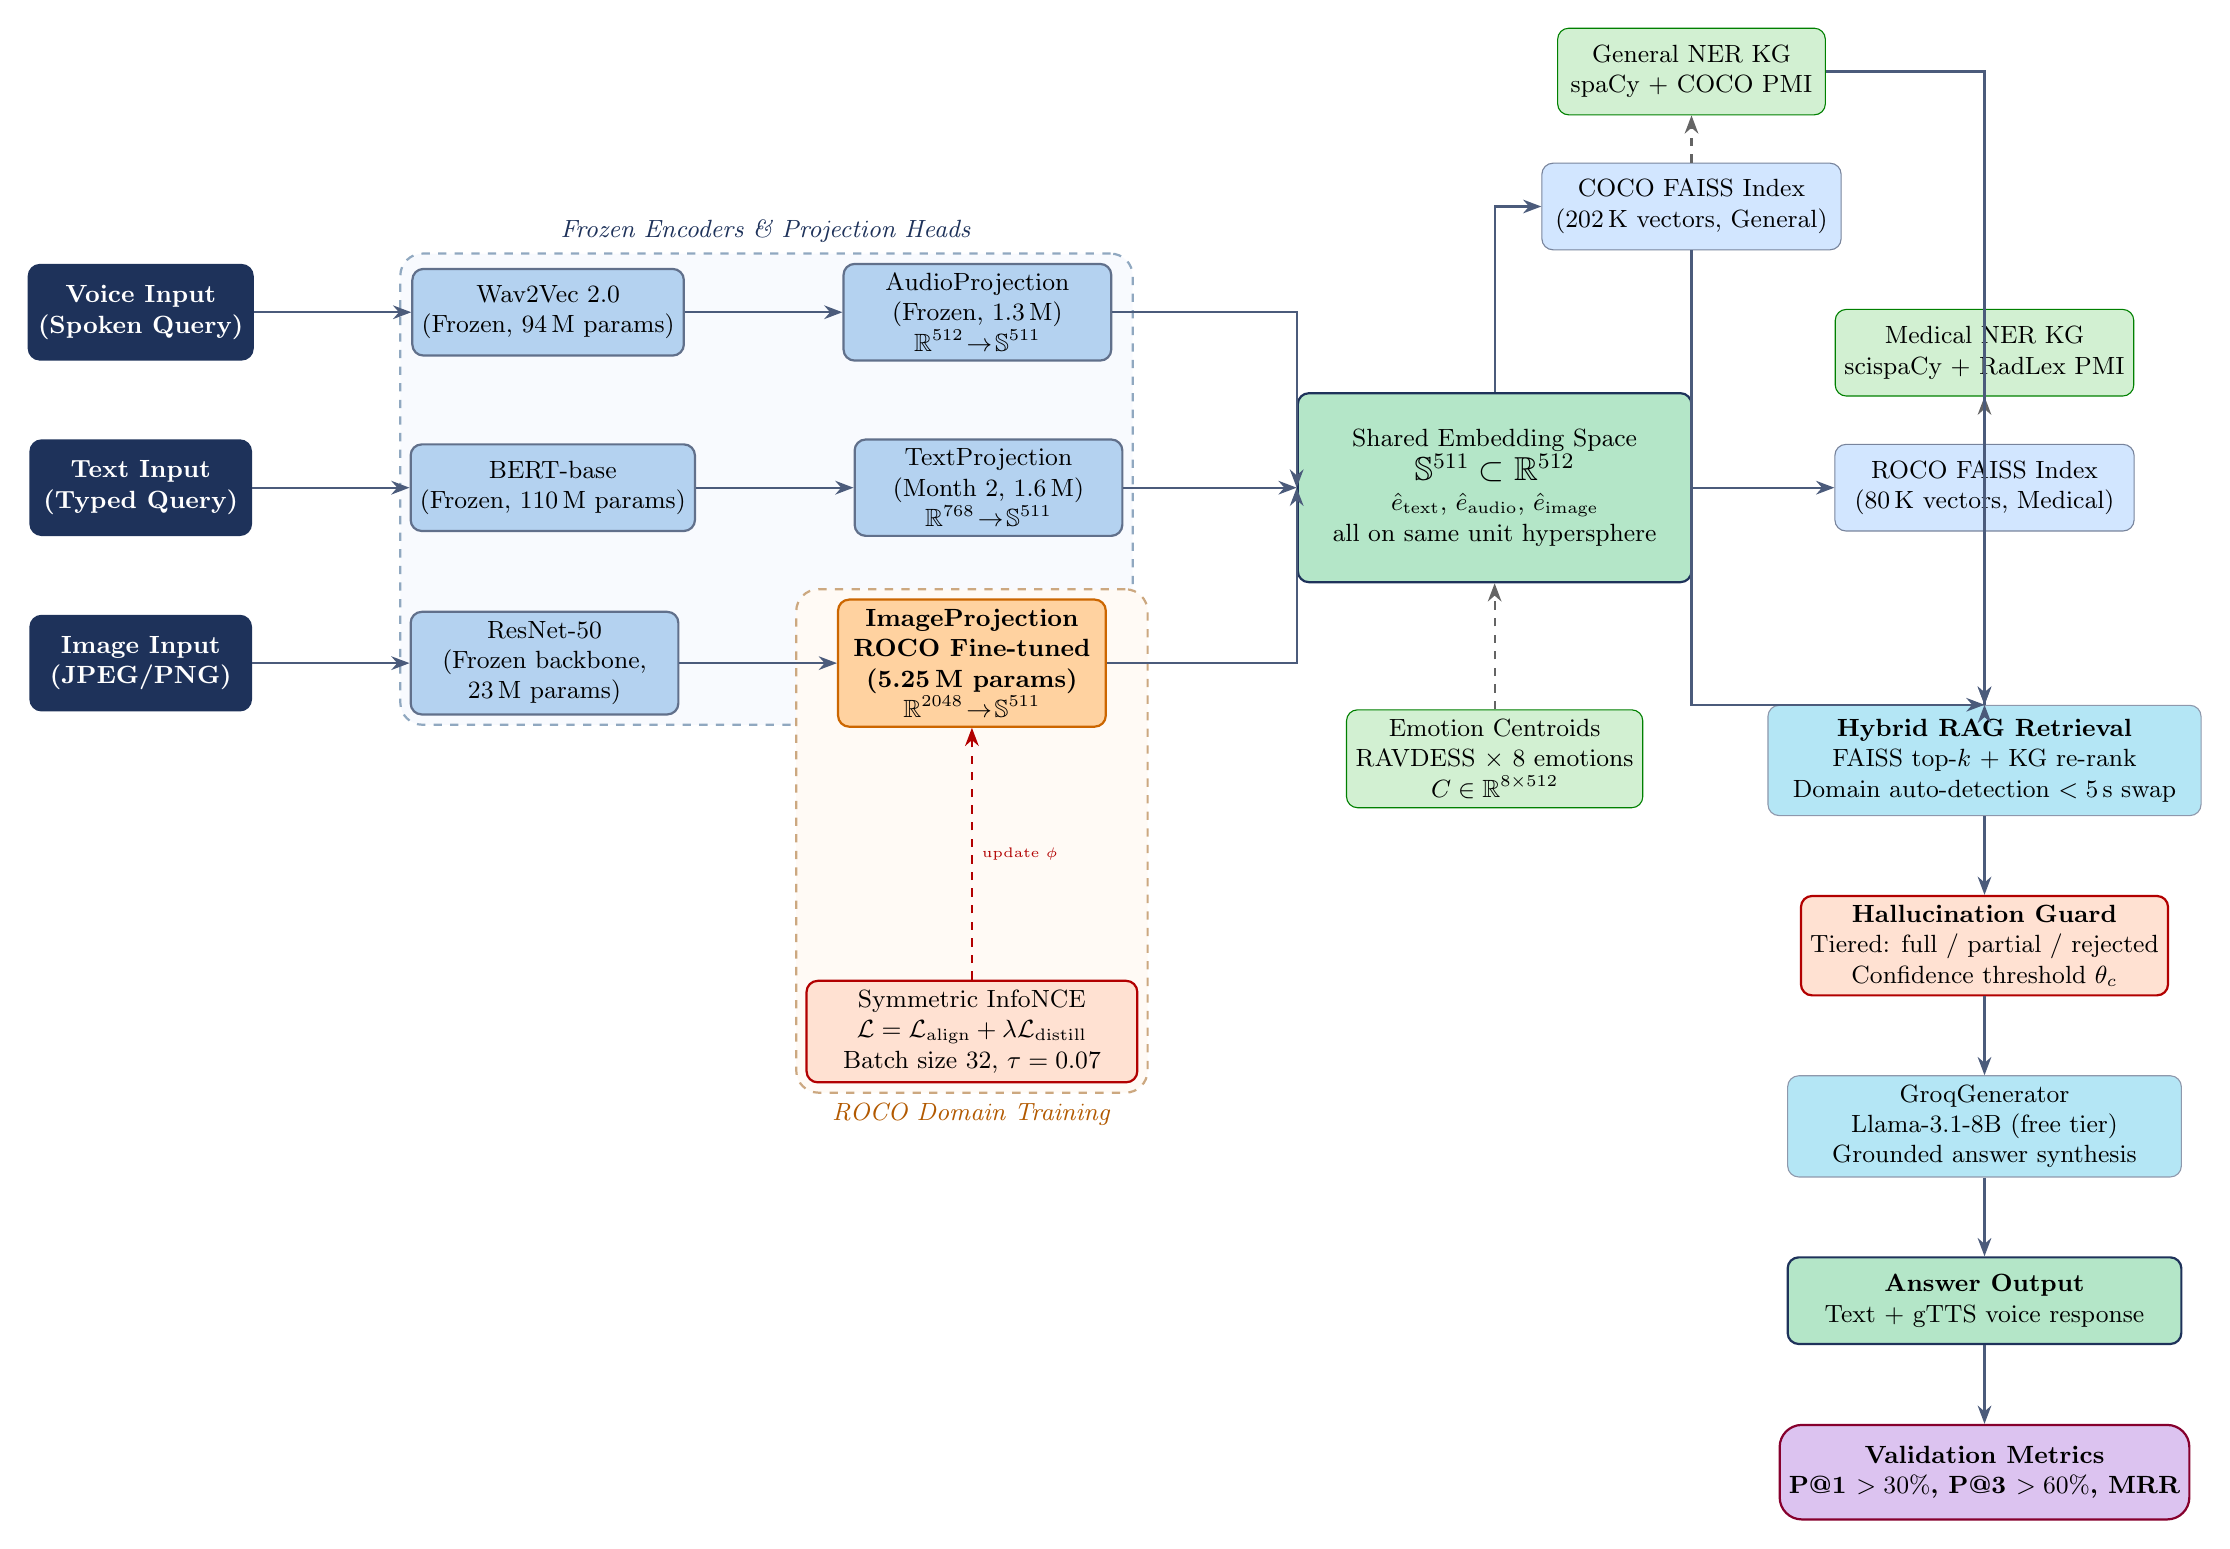
\begin{tikzpicture}[
  node distance=0.8cm and 1.2cm,
  >=Stealth,
  %--- Node styles
  inputbox/.style={rectangle, rounded corners=4pt, draw=darknavy, thick,
    fill=darknavy, text=white, minimum width=2.8cm, minimum height=1.2cm,
    align=center, font=\small\bfseries},
  frozenbox/.style={rectangle, rounded corners=4pt, draw=darknavy!70, thick,
    fill=frozenblue, minimum width=3.4cm, minimum height=1.1cm,
    align=center, font=\small},
  trainbox/.style={rectangle, rounded corners=4pt, draw=orange!80!black, thick,
    fill=trainableorange, minimum width=3.4cm, minimum height=1.1cm,
    align=center, font=\small\bfseries},
  outputbox/.style={rectangle, rounded corners=4pt, draw=darknavy, thick,
    fill=medicalgreen, minimum width=3.4cm, minimum height=1.1cm,
    align=center, font=\small},
  indexbox/.style={rectangle, rounded corners=4pt, draw=darknavy!60,
    fill=faisscolor, minimum width=3.8cm, minimum height=1.1cm,
    align=center, font=\small},
  kgbox/.style={rectangle, rounded corners=4pt, draw=green!50!black,
    fill=pmicolor, minimum width=3.4cm, minimum height=1.1cm,
    align=center, font=\small},
  lossbox/.style={rectangle, rounded corners=4pt, draw=red!70!black, thick,
    fill=infonce, minimum width=4cm, minimum height=1.1cm,
    align=center, font=\small},
  evalbox/.style={rectangle, rounded corners=8pt, draw=purple!70!black, thick,
    fill=cocoviolet, minimum width=4cm, minimum height=1.2cm,
    align=center, font=\small\bfseries},
  domainbox/.style={rectangle, rounded corners=4pt, draw=darknavy!50,
    fill=rococyan, minimum width=3.6cm, minimum height=1.1cm,
    align=center, font=\small},
  arrow/.style={->, thick, color=darknavy!80},
  dasharrow/.style={->, dashed, thick, color=midgray},
  redarrow/.style={->, thick, color=red!70!black},
]

%=== COLUMN 1: INPUTS ===
\node[inputbox] (voiceIn)  at (0,0)        {Voice Input\\\small(Spoken Query)};
\node[inputbox] (textIn)   [below=1cm of voiceIn]  {Text Input\\\small(Typed Query)};
\node[inputbox] (imageIn)  [below=1cm of textIn]   {Image Input\\\small(JPEG/PNG)};

%=== COLUMN 2: ENCODERS (FROZEN) ===
\node[frozenbox] (wav2vec)  [right=2cm of voiceIn]  {Wav2Vec 2.0\\\small(Frozen, 94\,M params)};
\node[frozenbox] (bert)     [right=2cm of textIn]   {BERT-base\\\small(Frozen, 110\,M params)};
\node[frozenbox] (resnet)   [right=2cm of imageIn]  {ResNet-50\\\small(Frozen backbone,\\23\,M params)};

%=== COLUMN 3: PROJECTION HEADS ===
\node[frozenbox] (audioproj)  [right=2cm of wav2vec]  {AudioProjection\\\small(Frozen, 1.3\,M)\\\small$\R^{512}\!\to\!\Sphere^{511}$};
\node[frozenbox] (textproj)   [right=2cm of bert]     {TextProjection\\\small(Month 2, 1.6\,M)\\\small$\R^{768}\!\to\!\Sphere^{511}$};
\node[trainbox]  (imageproj)  [right=2cm of resnet]   {ImageProjection\\\textbf{ROCO Fine-tuned}\\\small(5.25\,M params)\\\small$\R^{2048}\!\to\!\Sphere^{511}$};

%=== SHARED EMBEDDING SPACE ===
\node[outputbox, minimum width=5cm, minimum height=2.4cm]
     (embspace) [right=2.2cm of textproj]
     {Shared Embedding Space\\\large$\Sphere^{511} \subset \R^{512}$\\\small$\hat{e}_{\text{text}},\,\hat{e}_{\text{audio}},\,\hat{e}_{\text{image}}$\\\small all on same unit hypersphere};

%=== EMOTION CENTROIDS ===
\node[kgbox] (centroids) [below=1.6cm of embspace]
     {Emotion Centroids\\\small RAVDESS $\times$ 8 emotions\\\small$C \in \R^{8 \times 512}$};

%=== FAISS INDEX (two variants) ===
\node[indexbox] (cocoFAISS) [above=1.8cm of embspace, xshift=2.5cm]
     {COCO FAISS Index\\\small(202\,K vectors, General)};
\node[indexbox] (rocoFAISS) [right=1.8cm of embspace]
     {ROCO FAISS Index\\\small(80\,K vectors, Medical)};

%=== KNOWLEDGE GRAPHS ===
\node[kgbox] (kgGeneral) [above=0.6cm of cocoFAISS]
     {General NER KG\\\small spaCy + COCO PMI};
\node[kgbox] (kgMedical) [above=0.6cm of rocoFAISS]
     {Medical NER KG\\\small scispaCy + RadLex PMI};

%=== HYBRID RETRIEVAL ===
\node[domainbox, minimum width=5.5cm, minimum height=1.4cm]
     (retrieval) [below=2.2cm of rocoFAISS]
     {\textbf{Hybrid RAG Retrieval}\\\small FAISS top-$k$ $+$ KG re-rank\\\small Domain auto-detection $<5$\,s swap};

%=== HALLUCINATION GUARD ===
\node[lossbox] (hallguard) [below=1cm of retrieval]
     {\textbf{Hallucination Guard}\\\small Tiered: full / partial / rejected\\\small Confidence threshold $\theta_c$};

%=== LLM GENERATOR ===
\node[domainbox, minimum width=5cm] (groq) [below=1cm of hallguard]
     {GroqGenerator\\\small Llama-3.1-8B (free tier)\\\small Grounded answer synthesis};

%=== OUTPUT ===
\node[outputbox, minimum width=5cm] (answer) [below=1cm of groq]
     {\textbf{Answer Output}\\\small Text + gTTS voice response};

%=== INFONCE LOSS (training feedback) ===
\node[lossbox, minimum width=4.2cm] (infonceloss)
     [below=3.2cm of imageproj]
     {Symmetric InfoNCE\\\small$\mathcal{L} = \mathcal{L}_{\text{align}} + \lambda\mathcal{L}_{\text{distill}}$\\\small Batch size 32, $\tau=0.07$};

%=== EVAL ===
\node[evalbox] (eval) [below=1cm of answer]
     {Validation Metrics\\\small P@1 $>30\%$, P@3 $>60\%$, MRR};

%--- ARROWS: inputs to encoders
\draw[arrow] (voiceIn)  -- (wav2vec);
\draw[arrow] (textIn)   -- (bert);
\draw[arrow] (imageIn)  -- (resnet);

%--- ARROWS: encoders to projections
\draw[arrow] (wav2vec) -- (audioproj);
\draw[arrow] (bert)    -- (textproj);
\draw[arrow] (resnet)  -- (imageproj);

%--- ARROWS: projections to shared space
\draw[arrow] (audioproj) -| (embspace.west);
\draw[arrow] (textproj)  -- (embspace.west);
\draw[arrow] (imageproj) -| (embspace.west);

%--- ARROWS: shared space to indexes
\draw[arrow] (embspace.north) |- (cocoFAISS.west);
\draw[arrow] (embspace.east)  -- (rocoFAISS.west);

%--- ARROWS: indexes to KGs
\draw[dasharrow] (cocoFAISS) -- (kgGeneral);
\draw[dasharrow] (rocoFAISS) -- (kgMedical);

%--- ARROWS: to retrieval
\draw[arrow] (cocoFAISS.south) |- (retrieval.north);
\draw[arrow] (rocoFAISS.south) -- (retrieval.north);
\draw[arrow] (kgGeneral.east)  -| (retrieval.north);
\draw[arrow] (kgMedical.north) |- (retrieval.north);

%--- ARROWS: centroids to embspace
\draw[dasharrow] (centroids.north) -- (embspace.south);

%--- ARROWS: retrieval pipeline
\draw[arrow] (retrieval)  -- (hallguard);
\draw[arrow] (hallguard)  -- (groq);
\draw[arrow] (groq)       -- (answer);
\draw[arrow] (answer)     -- (eval);

%--- TRAINING FEEDBACK
\draw[redarrow, dashed] (infonceloss.north) -- (imageproj.south)
      node[midway, right, font=\tiny, color=red!70!black] {update $\phi$};

%--- BOUNDING BOXES for sections
\begin{pgfonlayer}{background}
  \node[draw=frozenblue!80!black, thick, dashed, fill=frozenblue!10,
        rounded corners=8pt, fit=(wav2vec)(bert)(resnet)(audioproj)(textproj),
        label={[font=\small,color=darknavy]above:\textit{Frozen Encoders \& Projection Heads}}]
        (frozenGroup) {};
  \node[draw=trainableorange!80!black, thick, dashed, fill=trainableorange!10,
        rounded corners=8pt, fit=(imageproj)(infonceloss),
        label={[font=\small,color=orange!70!black]below:\textit{ROCO Domain Training}}]
        (trainGroup) {};
\end{pgfonlayer}

\end{tikzpicture}%
}
\caption{MIVA-KNIGHT Month 4 full pipeline. Blue boxes: frozen components. Orange boxes: retrained. Green boxes: outputs/metrics. Cyan boxes: retrieval and generation. Red dashed arrow: training gradient update to ImageProjection only.}
\label{fig:pipeline}
\end{figure}

%=============================================================================
\section{Mathematical Foundations}
\label{sec:math}

\subsection{The Unit Hypersphere}

\begin{definition}[Unit Hypersphere $\Sphere^{511}$]
The $(512-1)$-dimensional unit hypersphere is
\[
\Sphere^{511} = \left\{ v \in \R^{512} \;\Big|\; \norm{v} = 1 \right\}.
\]
All MIVA-KNIGHT embeddings are constrained to $\Sphere^{511}$ via L2-normalisation.
\end{definition}

\begin{axiom}[L2-Normalisation]
For any vector $x \in \R^{512}$, the L2-normalised vector is
\[
\hat{x} = \frac{x}{\norm{x}}, \qquad \hat{x} \in \Sphere^{511}.
\]
\end{axiom}

\begin{theorem}[Cosine = Inner Product on $\Sphere^{511}$]
For $\hat{u}, \hat{v} \in \Sphere^{511}$, cosine similarity equals their inner product:
\[
\cos(\hat{u}, \hat{v}) = \frac{\hat{u} \cdot \hat{v}}{\norm{\hat{u}}\norm{\hat{v}}} = \hat{u} \cdot \hat{v}.
\]
\end{theorem}

\begin{proof}
Since $\norm{\hat{u}} = \norm{\hat{v}} = 1$ by definition of the unit hypersphere, the denominator equals $1 \cdot 1 = 1$, so cosine similarity reduces to the inner product. \qed
\end{proof}

\layman{Imagine all meaning-fingerprints pinned on the surface of a giant balloon in 512-dimensional space. ``Closeness'' is measured by the angle between two pins. Because all pins are on the surface (unit distance from centre), the angle formula simplifies to a plain dot product --- making similarity computation extremely fast.}

%=============================================================================
\section{Step 1: Smoke Test (Fail-Fast Principle)}
\label{sec:smoketest}

\subsection{Purpose}

A \emph{smoke test} is a minimal, fast verification that the entire system infrastructure is intact before committing to expensive computation.

\begin{theorem}[Fail-Fast Minimises Wasted Compute]
\label{thm:failfast}
Let $T_{\text{detect}}$ be the time to detect an infrastructure failure, and $T_{\text{waste}}$ the compute consumed before detection. For failures caught at module import time: $T_{\text{detect}} < 10\,\text{s}$, $T_{\text{waste}} \approx 0\,\text{GPU-seconds}$. For failures caught after model loading: $T_{\text{detect}} \approx 45\,\text{s}$, $T_{\text{waste}} \approx 3\,\text{GB VRAM}$.
\end{theorem}

\begin{algorithm}[H]
\caption{SMOKE\_TEST --- Pre-flight Infrastructure Verification}
\label{alg:smoketest}
\begin{algorithmic}[1]
\Require \texttt{MODULE\_DIR} appended to \texttt{sys.path}
\Ensure System ready for full pipeline, or specific error message
\State \textbf{Try} \texttt{from pipeline import MIVAKnight, TextQuery}
  \Comment{Tests: torch, transformers, faiss importable}
\State \textbf{Try} \texttt{from domain\_config import GeneralDomain, MedicalDomain}
  \Comment{Tests: RadLex seed list defined, no syntax errors}
\State \textbf{Try} \texttt{from generator import GroqGenerator}
  \Comment{Tests: groq package installed}
\State $\textit{device} \gets \texttt{torch.cuda.is\_available()} \;?\; \texttt{'cuda'} : \texttt{'cpu'}$
\State \textbf{Print} $\texttt{"=== Smoke test passed ==="} \;\|\; \textit{device}$
\end{algorithmic}
\end{algorithm}

\layman{Before a pilot takes off, they run a 20-minute pre-flight checklist: fuel, instruments, communications. This smoke test is that checklist compressed to 10 seconds. Failing here costs 10 seconds; failing after loading 235 million parameters costs 45 minutes.}

%=============================================================================
\section{Step 2: Emotion Centroid Computation}
\label{sec:centroids}

\subsection{Motivation}

MIVA-KNIGHT enriches text queries with emotional context from the RAVDESS audio database (1,440 clips, 8 emotions, 24 actors). Pre-computing a single representative \emph{spherical centroid} per emotion class reduces inference lookup to microseconds.

\subsection{AudioProjection Architecture}

\begin{definition}[AudioProjection]
The AudioProjection $f_\theta: \R^{512} \to \Sphere^{511}$ is a two-layer MLP:
\[
f_\theta(x) = \text{L2-norm}\!\left(\text{LN}_{512}\!\left(W_2 \cdot \text{GELU}\!\left(\text{LN}_{512}(W_1 x + b_1)\right) + b_2\right)\right)
\]
where $W_1, W_2 \in \R^{512 \times 512}$. Total parameters: $\approx 1.3\,\text{M}$.
\end{definition}

\begin{definition}[Spherical Centroid]
For emotion class $e$ with $N_e$ projected audio embeddings $\{\hat{a}_1^{(e)}, \ldots, \hat{a}_{N_e}^{(e)}\} \subset \Sphere^{511}$, the spherical centroid is:
\[
\bar{c}_e = \frac{\mu_e}{\norm{\mu_e}}, \qquad \mu_e = \frac{1}{N_e}\sum_{i=1}^{N_e} \hat{a}_i^{(e)} \in \R^{512}.
\]
\end{definition}

\begin{lemma}[Centroid Optimality on $\Sphere^{511}$]
\label{lem:centroid}
The spherical centroid $\bar{c}_e$ is the point on $\Sphere^{511}$ that minimises the sum of squared geodesic distances to all class members:
\[
\bar{c}_e = \arg\min_{v \in \Sphere^{511}} \sum_{i=1}^{N_e} \arccos^2\!\left(\hat{a}_i^{(e)} \cdot v\right).
\]
\end{lemma}

\begin{proof}[Proof sketch]
Minimising $\sum_i \arccos^2(\hat{a}_i \cdot v)$ over $v \in \Sphere^{511}$ is equivalent (for small angles) to minimising $\sum_i \norm{\hat{a}_i - v}^2$ subject to $\norm{v}=1$. The unconstrained minimiser of the sum of squared Euclidean distances is the Euclidean mean $\mu_e$; projecting back onto $\Sphere^{511}$ via L2-normalisation gives $\bar{c}_e$. \qed
\end{proof}

\begin{algorithm}[H]
\caption{BUILD\_EMOTION\_CENTROIDS}
\label{alg:centroids}
\begin{algorithmic}[1]
\Require \texttt{AUDIO\_PROJ\_PATH}, \texttt{RAVDESS\_CACHE}
\Ensure \texttt{emotion\_centroids.pt} $\in \R^{8 \times 512}$
\State Load AudioProjection weights; set \texttt{projection.eval()}
\State Load RAVDESS cache: 1,440 entries \texttt{\{filename $\to$ \{embedding, emotion\}\}}
\For{each entry $(\text{filename}, \text{data})$ in cache}
  \State $\text{emb} \gets \text{data['embedding']}.\text{to(device)}$ \Comment{$[512]$}
  \State $\hat{a} \gets f_\theta(\text{emb})$ (no gradient) \Comment{$\hat{a} \in \Sphere^{511}$}
  \State \texttt{emotion\_embs[data['emotion']]}.append($\hat{a}$)
\EndFor
\For{each emotion $e \in \{\text{angry, calm, disgust, fearful, happy, neutral, sad, surprised}\}$}
  \State $\mu_e \gets \frac{1}{N_e}\sum \hat{a}_i^{(e)}$ \Comment{Euclidean mean, $\in \R^{512}$}
  \State $\bar{c}_e \gets \mu_e / \norm{\mu_e}$ \Comment{Project to $\Sphere^{511}$}
\EndFor
\State \texttt{torch.save}(stack($\bar{c}_e$), \texttt{CENTROIDS\_PATH}) \Comment{Shape $[8, 512]$}
\end{algorithmic}
\end{algorithm}

\layman{Imagine 180 people each pointing their arm in slightly different directions to indicate ``happy.'' The centroid is the single average direction that best represents all 180 arms. At query time the system asks: ``which of 8 emotion-directions does this question most resemble?'' in microseconds, rather than re-processing 1,440 audio clips every time.}

%=============================================================================
\section{Step 3: ROCO Dataset Download and Persistence}
\label{sec:roco}

\subsection{The ROCO Dataset}

ROCO (Radiology Objects in COntext) is a public medical image-caption dataset of $\approx$81\,K X-ray images paired with author-written clinical captions from PubMed Open Access articles.

\begin{algorithm}[H]
\caption{DOWNLOAD\_AND\_CACHE\_ROCO}
\label{alg:roco}
\begin{algorithmic}[1]
\Require HuggingFace ID: \texttt{eltorio/ROCOv2}
\Ensure All images and metadata persisted to Google Drive
\If{\texttt{roco\_train\_metadata.json} already exists on Drive}
  \State \textbf{Print} ``[SKIP] Already cached: $N$ samples''; \Return \Comment{Idempotent guard}
\EndIf
\State $\texttt{roco\_train} \gets \text{load\_dataset}(\ldots, \text{split}=\text{``train''})$
\State $\texttt{roco\_val} \gets \text{load\_dataset}(\ldots, \text{split}=\text{``validation''})$
\Procedure{SaveSplit}{$\textit{dataset}, \textit{split\_name}$}
  \For{$(i, \text{item}) \in \text{enumerate}(\textit{dataset})$}
    \State $\textit{img\_path} \gets \texttt{ROCO\_CACHE/images/\{split\_name\}\_\{i:06d\}.jpg}$
    \If{$\textit{img\_path}$ not on disk}
      \State \texttt{item['image'].save(img\_path)} \Comment{Persist PIL JPEG}
    \EndIf
    \State $\textit{meta} \mathrel{+}= \{$\texttt{doc\_id}, \texttt{text}, \texttt{image\_path}$\}$
  \EndFor
  \State \texttt{json.dump(meta, \ldots)}
\EndProcedure
\State \Call{SaveSplit}{\texttt{roco\_train}, \texttt{'train'}} \Comment{$\approx$60\,K iterations}
\State \Call{SaveSplit}{\texttt{roco\_val}, \texttt{'validation'}} \Comment{$\approx$20\,K iterations}
\end{algorithmic}
\end{algorithm}

\layman{ROCO is the medical textbook library being added to the system. This step downloads 81,000 radiology images (like ordering books from a publisher) and saves everything to Google Drive, so the 8\,GB collection survives the Colab session ending. The metadata JSON files are the library catalogue: each book's reference number, its caption, and its shelf location on Drive.}

%=============================================================================
\section{Step 4: COCO FAISS Index and General Knowledge Graph}
\label{sec:coco}

\subsection{The Text Encoding Pipeline}

Every caption passes through an identical pipeline at index-build time and at query time, ensuring consistency:

\[
\text{caption}
\xrightarrow{\text{tokenise}} [t_1,\ldots,t_T]
\xrightarrow{\text{BERT}} H^{(12)} \in \R^{T \times 768}
\xrightarrow{\text{mean pool}} e_{\text{bert}} \in \R^{768}
\xrightarrow{\text{TextProjection}} \xrightarrow{\text{L2-norm}}
\hat{e} \in \Sphere^{511}
\]

\subsection{FAISS IndexFlatIP}

\begin{definition}[FAISS IndexFlatIP]
\texttt{IndexFlatIP} stores all $N$ embeddings as a dense float32 matrix $\mathbf{E} \in \R^{N \times 512}$ and performs exact inner-product search:
\[
\text{top-}k(q) = \arg\text{sort}_{j}\!\left(-\mathbf{E}\,q^\top\right)[{:k}].
\]
For L2-normalised vectors, $\mathbf{E}\,q^\top$ gives exact cosine similarities by Axiom 1.
\end{definition}

\begin{theorem}[FAISS Complexity and Correctness]
For $N$ unit vectors of dimension $D$, \texttt{IndexFlatIP} achieves:
\begin{itemize}
  \item \textbf{Time:} $\mathcal{O}(N \cdot D)$ per query via BLAS GEMM with AVX2 SIMD.
  \item \textbf{Recall:} 100\% (exact search, no approximation error).
  \item \textbf{Practical:} $N=200{,}000$, $D=512$ $\Rightarrow$ $\approx 0.5\,\text{ms}$ per query on CPU.
\end{itemize}
\end{theorem}

\begin{algorithm}[H]
\caption{BUILD\_COCO\_FAISS\_INDEX}
\label{alg:coco_faiss}
\begin{algorithmic}[1]
\Require \texttt{captions\_val2017.json} (202,654 annotations), TextProjection weights
\Ensure \texttt{coco\_val2017.faiss}, \texttt{coco\_corpus\_metadata.json}
\If{\texttt{COCO\_FAISS} and \texttt{COCO\_META} exist}
  \State \textbf{Print} ``[SKIP] COCO FAISS index already exists''; \Return
\EndIf
\State Build $\textit{corpus\_meta}$: for each $(img\_id, caption)$, record \texttt{doc\_id}, \texttt{text}, \texttt{image\_path}
\Procedure{EncodeTexts}{$\textit{texts}$, $\textit{batch\_size}=256$}
  \For{$i = 0$ \textbf{to} $|\textit{texts}|$ \textbf{step} $256$}
    \State $\textit{inp} \gets \text{tokeniser}(\textit{batch},\, \texttt{max\_length}=128,\, \texttt{padding},\, \texttt{truncation})$
    \State $e_{\text{bert}} \gets \text{BERT}(\textit{inp}).\text{last\_hidden\_state.mean(dim=1)}$ \Comment{$[256, 768]$}
    \State $\hat{e} \gets \text{L2-norm}(\text{TextProjection}(e_{\text{bert}}))$ \Comment{$[256, 512]$}
    \State Accumulate $\hat{e}$
  \EndFor
  \State \Return $\texttt{torch.cat}(\cdot)$ \Comment{$[N, 512]$}
\EndProcedure
\State $\textit{embs} \gets \Call{EncodeTexts}{\textit{texts}}$
\State $\textit{index} \gets \texttt{faiss.IndexFlatIP}(512)$
\State $\textit{index}.\text{add}(\textit{embs}.\text{numpy}().\text{astype}(\texttt{'float32'}))$
\State \texttt{faiss.write\_index}($\textit{index}$, \texttt{COCO\_FAISS})
\end{algorithmic}
\end{algorithm}

\subsection{Pointwise Mutual Information Knowledge Graph}

\begin{definition}[Pointwise Mutual Information (PMI)]
For entities $a$ and $b$ co-occurring in a corpus of $N$ documents:
\[
\text{PMI}(a, b) = \log \frac{P(a,b)}{P(a) \cdot P(b)} = \log \frac{c_{ab} \cdot N}{f_a \cdot f_b},
\]
where $c_{ab}$ = co-occurrence count, $f_a$, $f_b$ = individual document frequencies.
\end{definition}

\begin{axiom}[PMI Semantic Association]
$\text{PMI}(a,b) > 0$ if and only if entities $a$ and $b$ co-occur more frequently than would be expected under statistical independence, indicating genuine semantic association.
\end{axiom}

\begin{example}[PMI Calculation]
Let $N = 200{,}000$, $f_{\text{dog}} = 8{,}000$, $f_{\text{leash}} = 1{,}200$, $c_{\text{dog,leash}} = 900$:
\[
\text{PMI}(\text{dog}, \text{leash}) = \log\!\frac{900 \times 200{,}000}{8{,}000 \times 1{,}200} = \log(18.75) \approx 2.93.
\]
High PMI confirms strong semantic association.
\end{example}

\begin{definition}[General NER Knowledge Graph $\KG_G$]
The general knowledge graph is a PMI-weighted undirected graph $\KG_G = (\mathcal{V}_G, \mathcal{E}_G, w)$ where:
\begin{itemize}
  \item $\mathcal{V}_G$ = top-2,000 most frequent entities from COCO captions (via spaCy noun chunks and named entities),
  \item $(a,b) \in \mathcal{E}_G$ iff $\text{PMI}(a,b) > 0$ and $c_{ab} \geq 3$,
  \item $w(a,b) = \text{PMI}(a,b)$.
\end{itemize}
\end{definition}

\begin{algorithm}[H]
\caption{BUILD\_GENERAL\_NER\_KG}
\label{alg:kg_general}
\begin{algorithmic}[1]
\Require $N$ COCO captions, spaCy \texttt{en\_core\_web\_sm}
\Ensure \texttt{ner\_kg\_general.pkl}: $\texttt{dict}[\text{entity} \to \texttt{dict}[\text{entity} \to \text{PMI}]]$
\For{captions in batches of 1,000}
  \State $\textit{doc} \gets \texttt{nlp}(\textit{caption})$
  \State $\textit{ents} \gets \{\text{noun\_chunks}\} \cup \{\text{named\_entities}\}$ (lowercased)
  \State Append $\textit{ents}$ to $\textit{doc\_entities}$
\EndFor
\State $\textit{entity\_freq} \gets \texttt{Counter}(\bigcup \textit{doc\_entities})$
\State $\textit{top\_entities} \gets \text{top-}2000$ most frequent (min freq $\geq 5$)
\For{each document's entity set (filtered to $\textit{top\_entities}$)}
  \For{each symmetric pair $(a, b)$}
    \State $\textit{cooc}[a][b] \mathrel{+}= 1$;\quad $\textit{cooc}[b][a] \mathrel{+}= 1$
  \EndFor
\EndFor
\For{each $a$ with $\textit{entity\_freq}[a] \geq 5$}
  \For{each $(b, c_{ab})$ with $c_{ab} \geq 3$}
    \State $\textit{pmi} \gets \log\!\left(\frac{c_{ab} \cdot N}{f_a \cdot f_b + \epsilon}\right)$
    \If{$\textit{pmi} > 0$}
      \State $\textit{kg}[a][b] \gets \texttt{round}(\textit{pmi}, 4)$
    \EndIf
  \EndFor
\EndFor
\State \texttt{pickle.dump}(\textit{kg}, \texttt{KG\_GENERAL})
\end{algorithmic}
\end{algorithm}

\layman{PMI measures ``do these concepts travel together?'' If ``dog'' and ``leash'' appear in the same sentence far more often than chance, their PMI is high. Building the KG means reading 202,000 captions and noting every pair of concepts that co-appear frequently, scoring each by how surprising their co-occurrence is. At retrieval time, if someone asks about ``dog,'' the KG boosts documents mentioning ``leash,'' ``collar,'' and ``park'' --- related concepts the query didn't explicitly state.}

%=============================================================================
\section{Step 5: Fine-tuning ImageProjection on ROCO}
\label{sec:finetune}

\subsection{The Domain Transfer Problem}

\begin{definition}[Domain Transfer]
Let $\Emb \subset \Sphere^{511}$ be the shared embedding space from Month 2, where TextProjection $f_T$ maps captions such that related captions cluster together. Domain transfer trains $f_I^{\text{ROCO}}$ such that:
\[
f_I^{\text{ROCO}}\!\left(\text{ResNet}(\text{X-ray}_i)\right) \approx f_T(\text{caption}_i),
\qquad \forall\, i \in \text{ROCO training set},
\]
without significantly displacing text embeddings.
\end{definition}

\subsection{ImageProjection Architecture}

\begin{definition}[ImageProjection $f_\phi$]
\[
f_\phi: \R^{2048} \to \Sphere^{511}, \qquad
f_\phi(x) = \frac{g_\phi(x)}{\norm{g_\phi(x)}},
\]
\[
g_\phi(x) = \text{LN}_{512}\!\left(W_2 \cdot \text{GELU}\!\left(\text{LN}_{2048}(W_1 x + b_1)\right) + b_2\right),
\]
where $W_1 \in \R^{2048 \times 2048}$, $W_2 \in \R^{512 \times 2048}$. Total parameters: $\approx 5.25\,\text{M}$.
\end{definition}

\begin{remark}
ImageProjection mirrors TextProjection exactly --- same two-layer MLP, same GELU + LayerNorm + L2-norm. This architectural symmetry ensures both heads produce comparably-scaled representations for contrastive training.
\end{remark}

\subsection{ImageNet Normalisation --- Why It Matters}

\begin{axiom}[Mandatory ImageNet Normalisation]
Input images must be normalised per channel:
\[
\hat{x}_{c,h,w} = \frac{x_{c,h,w} - \mu_c}{\sigma_c}, \qquad
\mu = [0.485, 0.456, 0.406],\quad
\sigma = [0.229, 0.224, 0.225],
\]
where $\mu, \sigma$ are the per-channel mean and standard deviation of the ImageNet-1K training set. The ResNet-50 BatchNorm layers were calibrated with these exact statistics during pre-training. Any deviation shifts pool5 features off-distribution and degrades embedding quality.
\end{axiom}

\subsection{Symmetric InfoNCE Loss}

\begin{definition}[Symmetric InfoNCE Loss]
For a batch of $B = 32$ (caption, X-ray) pairs with temperature $\tau = 0.07$, and similarity matrix $S_{ij} = \hat{e}^{\text{text}}_i \cdot \hat{e}^{\text{image}}_j$:
\[
\mathcal{L}_{\text{InfoNCE}} = \frac{1}{2B}\sum_{i=1}^{B}\left[
  -\log\frac{\exp(S_{ii}/\tau)}{\sum_{j=1}^{B}\exp(S_{ij}/\tau)}
  -\log\frac{\exp(S_{ii}/\tau)}{\sum_{j=1}^{B}\exp(S_{ji}/\tau)}
\right].
\]
\end{definition}

\begin{theorem}[InfoNCE Random Baseline]
For a batch of size $B$ with a randomly initialised model (all $S_{ij}$ equal):
\[
\mathcal{L}_{\text{InfoNCE}}^{\text{random}} = \log B.
\]
For $B = 32$: $\mathcal{L}^{\text{random}} = \log 32 \approx 3.47$. Loss near this value after several epochs indicates the model is not learning.
\end{theorem}

\begin{proof}
Under a random model, $S_{ij} = c$ for all $i,j$. Then $\exp(S_{ii}/\tau) / \sum_j \exp(S_{ij}/\tau) = 1/B$ and $-\log(1/B) = \log B$. \qed
\end{proof}

\begin{definition}[Dual Loss with Knowledge Distillation]
The full training objective adds a distillation term to prevent catastrophic forgetting of the Month~2 text embedding structure:
\[
\mathcal{L}_{\text{total}} = \mathcal{L}_{\text{align}} + \lambda(t) \cdot \mathcal{L}_{\text{distill}},
\]
\[
\mathcal{L}_{\text{distill}} = \frac{1}{B}\sum_{i=1}^{B}\!\left\|
  f_T^{\text{ROCO}}(c_i) - f_T^{\text{M2}}(c_i)
\right\|_2^2,
\]
where $\lambda(t)$ is a warm-up schedule that starts high (preserving Month 2 space) and decays as ROCO alignment improves.
\end{definition}

\begin{algorithm}[H]
\caption{FINETUNE\_IMAGE\_PROJECTION (ROCO Domain Transfer)}
\label{alg:finetune}
\begin{algorithmic}[1]
\Require ROCO train metadata ($\approx$60\,K pairs), frozen TextProjection, frozen ResNet-50
\Ensure \texttt{image\_projection\_roco.pth}, optionally \texttt{text\_projection\_roco.pth}
\State Initialise fresh \texttt{ImageProjection} (random weights)
\State Load frozen BERT + TextProjection (Month 2)
\State Load frozen ResNet-50 backbone (ImageNet)
\State Optimiser $\gets$ AdamW(ImageProjection.params, lr=$5\times10^{-4}$)
\State TextOptimiser $\gets$ AdamW(TextProjection.params, lr=$1\times10^{-5}$) \Comment{Nudge only}
\For{epoch = 1 \textbf{to} 15}
  \For{each batch of $B=32$ (caption, image\_path) pairs}
    \State $\hat{e}_{\text{text}} \gets \text{L2-norm}(f_T(\text{BERT}(\text{tokenise}(c_i))))$ \Comment{$[B, 512]$}
    \State $\hat{e}_{\text{img}} \gets f_\phi(\text{ResNet}(\text{preprocess}(\text{img}_i)))$ \Comment{$[B, 512]$}
    \State $S \gets \hat{e}_{\text{text}} \cdot \hat{e}_{\text{img}}^\top$ \Comment{Similarity matrix $[B, B]$}
    \State $\mathcal{L} \gets \Call{SymmetricInfoNCE}{S, \tau=0.07}$
    \State Optionally add $\mathcal{L}_{\text{distill}}$ with warm-up weight $\lambda(t)$
    \State $\mathcal{L}.\text{backward}()$;\quad Optimiser.step()
  \EndFor
  \State Save best checkpoint based on validation loss
\EndFor
\State \texttt{torch.save}(ImageProjection.state\_dict(), \texttt{IMG\_PROJ\_ROCO})
\end{algorithmic}
\end{algorithm}

\begin{lemma}[Feature Generality of Pool5]
Deep convolutional features from ResNet-50's \texttt{AdaptiveAvgPool2d} layer (pool5, 2048-dim) encode domain-agnostic visual primitives (edges, textures, spatial relationships). The final fully-connected softmax layer encodes only ImageNet-specific taxonomy. Therefore, removing the FC layer and using pool5 features transfers better to radiology than 1000-class class probabilities.
\end{lemma}

\layman{Step 5 is like teaching the image-reading component to understand X-rays. The ``eyes'' (ResNet-50) already know how to see edges, shapes, and densities --- they learned this from 1.2 million photos. We only teach the ``translator'' (ImageProjection) to convert those visual signals into the correct position in the shared meaning space, near the clinical caption it should match. The training signal (InfoNCE) punishes the model whenever it places an X-ray close to the \emph{wrong} caption and rewards it for placing it close to the \emph{correct} one.}

%=============================================================================
\section{Step 6: ROCO FAISS Index (MedicalDomain)}
\label{sec:roco_faiss}

\begin{algorithm}[H]
\caption{BUILD\_ROCO\_FAISS\_INDEX}
\label{alg:roco_faiss}
\begin{algorithmic}[1]
\Require \texttt{roco\_train\_metadata.json}, \texttt{roco\_validation\_metadata.json},\\
         TextProjection (ROCO-nudged preferred, Month 2 fallback)
\Ensure \texttt{roco\_medical.faiss}, \texttt{roco\_corpus\_metadata.json}
\State \textbf{Fallback chain:}
\If{\texttt{text\_projection\_roco.pth} exists}
  \State Load ROCO-adapted TextProjection \Comment{Better medical vocabulary}
\Else
  \State Load Month 2 TextProjection \Comment{Fallback; still buildable}
\EndIf
\State $\textit{corpus} \gets \texttt{roco\_train} + \texttt{roco\_val}$ \Comment{$\approx$80\,K records}
\State $\textit{embs} \gets \Call{EncodeTexts}{\textit{corpus.texts}}$ \Comment{Algorithm \ref{alg:coco_faiss}}
\State $\textit{index} \gets \texttt{faiss.IndexFlatIP}(512)$
\State $\textit{index}.\text{add}(\textit{embs})$;\quad Save to \texttt{ROCO\_FAISS}
\end{algorithmic}
\end{algorithm}

\layman{This step creates the medical catalogue. Whereas the general library (COCO FAISS) holds 202,000 everyday image captions, the medical library (ROCO FAISS) holds 80,000 radiology captions. When a query arrives about ``pleural effusion,'' the system searches the medical library instead of the general one.}

%=============================================================================
\section{Step 7: Medical Knowledge Graph (scispaCy + RadLex)}
\label{sec:kg_medical}

\subsection{Motivation}

The general KG covers COCO everyday vocabulary. It cannot handle radiology-specific concepts because \texttt{en\_core\_web\_sm} does not identify ``bilateral consolidation'' or ``pleural effusion'' as named entities, and COCO captions contain none of these terms.

\begin{definition}[Medical NER Knowledge Graph $\KG_M$]
$\KG_M = (\mathcal{V}_M, \mathcal{E}_M, w)$ where:
\begin{itemize}
  \item $\mathcal{V}_M$ = top-3,000 entities by frequency \emph{union} all RadLex seeds,
  \item $(a,b) \in \mathcal{E}_M$ iff $\text{PMI}(a,b) > 0$ and $c_{ab} \geq 2$,
  \item $w(a,b) = \text{PMI}(a,b)$.
\end{itemize}
\end{definition}

\begin{theorem}[RadLex Seed Coverage Guarantee]
By forcing all RadLex seed terms into $\mathcal{V}_M$ regardless of corpus frequency, critical imaging terms (e.g.\ \emph{pneumothorax}, \emph{cardiomegaly}) are guaranteed to be present in the KG even if they appear rarely in the ROCO validation split.
\end{theorem}

\begin{algorithm}[H]
\caption{BUILD\_MEDICAL\_NER\_KG}
\label{alg:kg_medical}
\begin{algorithmic}[1]
\Require $\approx$80\,K ROCO captions, scispaCy \texttt{en\_core\_sci\_sm}, \texttt{RADLEX\_SEEDS}
\Ensure \texttt{ner\_kg\_medical.pkl}
\For{each caption in batches of 1,000}
  \State $\textit{ents} \gets \{\text{noun\_chunk.lower()}\} \cup \{\text{ent.text.lower()}\}$ (scispaCy)
  \State $\textit{ents} \mathrel{\cup}= \{\textit{seed} \in \texttt{RADLEX\_SEEDS} : \textit{seed} \in \text{caption.lower()}\}$
  \State Append $\textit{ents}$ to $\textit{doc\_entities}$
\EndFor
\State $\textit{entity\_freq} \gets \texttt{Counter}(\bigcup \textit{doc\_entities})$
\State $\textit{top\_entities} \gets \text{top-}3000 \cup \texttt{RADLEX\_SEEDS}$
\For{each document's entity set (filtered to $\textit{top\_entities}$)}
  \For{each symmetric pair $(a,b)$}
    \State $\textit{cooc}[a][b] \mathrel{+}= 1$;\quad $\textit{cooc}[b][a] \mathrel{+}= 1$
  \EndFor
\EndFor
\For{each $a$, $b$ with $c_{ab} \geq 2$}
  \State $\textit{pmi} \gets \log\!\left(\frac{c_{ab} \cdot N}{f_a \cdot f_b + \epsilon}\right)$
  \If{$\textit{pmi} > 0$}
    \State $\textit{kg}[a][b] \gets \textit{pmi}$
  \EndIf
\EndFor
\State \texttt{pickle.dump}(\textit{kg}, \texttt{KG\_MEDICAL})
\end{algorithmic}
\end{algorithm}

\layman{The general knowledge graph knows that ``dogs'' and ``leashes'' go together. The medical knowledge graph knows that ``pleural effusion'' and ``heart failure'' go together, that ``consolidation'' relates to ``pneumonia,'' and that ``cardiomegaly'' relates to ``cardiac enlargement.'' This medical dictionary is built by reading 80,000 radiology captions and measuring which medical terms appear together most often.}

%=============================================================================
\section{Step 8: Validation --- Domain Transfer Evaluation}
\label{sec:eval}

\subsection{Domain Auto-Swap Mechanism}

\begin{definition}[Domain Auto-Detection]
The pipeline's domain classifier detects RadLex-seed terms in a query. If any term from \texttt{MedicalDomain.domain\_entity\_list} is found but absent from \texttt{GeneralDomain.domain\_entity\_list}, the query is classified as medical, triggering a domain swap in under 5 seconds.
\end{definition}

\subsection{Retrieval Metrics}

\begin{definition}[Precision at $k$ (P@$k$)]
For a query with ground-truth document ID $d^*$:
\[
P@k = \frac{|\{d^*\} \cap \text{top-}k|}{k} = \begin{cases} 1/k & \text{if } d^* \in \text{top-}k \\ 0 & \text{otherwise} \end{cases}.
\]
Over a test set: $\overline{P@k} = \frac{1}{N_{\text{test}}} \sum_{i=1}^{N_{\text{test}}} P@k_i$.
\end{definition}

\begin{definition}[Mean Reciprocal Rank (MRR)]
\[
\text{MRR} = \frac{1}{N_{\text{test}}} \sum_{i=1}^{N_{\text{test}}} \frac{1}{\text{rank}_i},
\]
where $\text{rank}_i$ is the position of the correct document in the ranked retrieval list. $\text{MRR} = 1$ means the correct document is always ranked first.
\end{definition}

\begin{axiom}[Self-Retrieval Protocol]
Each ROCO validation caption is used as its own query. Since the ROCO FAISS index contains both train and validation captions, the correct document exists in the searchable pool. Success is measured by whether the ground-truth \texttt{doc\_id} appears in top-$k$ results.
\end{axiom}

\begin{algorithm}[H]
\caption{EVALUATE\_ROCO\_RETRIEVAL}
\label{alg:eval}
\begin{algorithmic}[1]
\Require \texttt{pipeline}, \texttt{val\_meta} (ROCO validation), $n=500$ samples
\Ensure \texttt{month4\_results.json} with P@1, P@3, MRR, domain swap time
\State Sample $n$ records from \texttt{val\_meta}
\State $\textit{hits}@1 \gets 0$;\quad $\textit{hits}@3 \gets 0$;\quad $\textit{rr\_sum} \gets 0$
\For{each record $(i, \text{item})$}
  \State $q \gets \text{item}[\texttt{'text'}]$;\quad $\textit{true\_id} \gets \text{item}[\texttt{'doc\_id'}]$
  \State $\textit{results} \gets \text{pipeline.retrieve}(q,\, k=3)$
  \State $\textit{top\_ids} \gets [\text{r}[\texttt{'doc\_id'}] \text{ for r in results}]$
  \If{$\textit{true\_id} = \textit{top\_ids}[0]$}
    \State $\textit{hits}@1 \mathrel{+}= 1$
  \EndIf
  \If{$\textit{true\_id} \in \textit{top\_ids}$}
    \State $\textit{hits}@3 \mathrel{+}= 1$
  \EndIf
  \State $\textit{rank} \gets \textit{top\_ids}.\text{index}(\textit{true\_id}) + 1$ if found else $\infty$
  \State $\textit{rr\_sum} \mathrel{+}= 1/\textit{rank}$
\EndFor
\State P@1 $\gets \textit{hits}@1 / n$;\quad P@3 $\gets \textit{hits}@3 / n$;\quad MRR $\gets \textit{rr\_sum} / n$
\State Time domain swap; verify $< 5\,\text{s}$
\State Write \texttt{month4\_results.json}
\end{algorithmic}
\end{algorithm}

\begin{table}[h]
\centering
\caption{Month 4 Validation Targets}
\label{tab:targets}
\begin{tabular}{llll}
\toprule
\textbf{Metric} & \textbf{Domain} & \textbf{Target} & \textbf{Interpretation} \\
\midrule
P@3             & General (COCO)  & $\geq 55\%$ & Regression guard from Month 2 \\
P@1             & Medical (ROCO)  & $> 30\%$   & First domain-transfer baseline \\
P@3             & Medical (ROCO)  & $> 60\%$   & Clinical shortlisting recall at 3 \\
Domain swap     & Both            & $< 5\,\text{s}$ & Real-time interactive usability \\
\bottomrule
\end{tabular}
\end{table}

\layman{The evaluation is like a library retrieval test: each of 500 medical captions is given to the system as a query, and the system must find that exact caption's record in its 80,000-document database. P@1 asks ``was the correct record the very first result?''; P@3 asks ``was it in the top 3?''. Scoring above 30\% on P@1 for medical images is a meaningful baseline because the system has never seen radiology before Month 4, and the sheer variety of X-ray conditions makes exact retrieval challenging.}

%=============================================================================
\section{The Hybrid RAG Pipeline at Inference}
\label{sec:rag}

\subsection{Full Inference Algorithm}

\begin{algorithm}[H]
\caption{MIVA\_KNIGHT\_INFERENCE (Full Pipeline)}
\label{alg:inference}
\begin{algorithmic}[1]
\Require Voice/text query $q$, optional image $\mathcal{I}$, pipeline state
\Ensure Spoken + text answer grounded in retrieved documents
\Statex \textbf{Stage 1: Input Encoding}
\If{$q$ is audio}
  \State $q_{\text{text}} \gets \text{Whisper}(q)$ \Comment{Speech-to-text}
\EndIf
\State $\hat{e}_{\text{text}} \gets \text{L2-norm}(f_T(\text{BERT}(q_{\text{text}})))$
\State $\hat{e}_{\text{emotion}} \gets \bar{c}_{\arg\max_e (\hat{e}_{\text{text}} \cdot \bar{c}_e)}$
\If{image $\mathcal{I}$ provided}
  \State $\hat{e}_{\text{img}} \gets f_\phi(\text{ResNet}(\mathcal{I}))$ (domain-appropriate $f_\phi$)
  \State $\hat{e}_{\text{query}} \gets \text{L2-norm}(\alpha \hat{e}_{\text{text}} + \beta \hat{e}_{\text{img}} + \gamma \hat{e}_{\text{emotion}})$
\Else
  \State $\hat{e}_{\text{query}} \gets \text{L2-norm}(\hat{e}_{\text{text}} + \gamma \hat{e}_{\text{emotion}})$
\EndIf
\Statex \textbf{Stage 2: Domain Detection and Swap}
\If{$q_{\text{text}}$ contains RadLex seed terms}
  \State \Call{SwapDomain}{\texttt{MedicalDomain()}} \Comment{$< 5\,\text{s}$}
\EndIf
\Statex \textbf{Stage 3: FAISS Retrieval}
\State $(\textit{scores}, \textit{idxs}) \gets \textit{index}.\text{search}(\hat{e}_{\text{query}}, k=10)$
\Statex \textbf{Stage 4: KG Re-ranking}
\State Extract entities $\mathcal{Q}$ from $q_{\text{text}}$ via NER
\For{each retrieved doc $d_j$}
  \State $\textit{kg\_boost}(d_j) \gets \sum_{a \in \mathcal{Q}} \sum_{b \in \textit{doc\_entities}(d_j)} w_{\KG}(a,b)$
  \State $\textit{final\_score}(d_j) \gets \textit{scores}[j] + \delta \cdot \textit{kg\_boost}(d_j)$
\EndFor
\State $\textit{top\_k} \gets$ top-5 by $\textit{final\_score}$
\Statex \textbf{Stage 5: Hallucination Guard}
\State $c \gets \text{mean}(\textit{scores for top\_k})$
\If{$c \geq \theta_{\text{full}}$}
  \State confidence $\gets$ ``full''
\ElsIf{$c \geq \theta_{\text{partial}}$}
  \State confidence $\gets$ ``partial''
\Else
  \State confidence $\gets$ ``rejected''; \Return ``I cannot confidently answer.''
\EndIf
\Statex \textbf{Stage 6: LLM Answer Generation}
\State $\textit{prompt} \gets$ query + top-5 retrieved excerpts + confidence level
\State $\textit{answer} \gets \text{GroqGenerator}(\textit{prompt})$ \Comment{Llama-3.1-8B}
\Statex \textbf{Stage 7: Voice Output}
\State \texttt{gTTS}($\textit{answer}$).play() \Comment{Text-to-speech}
\State \Return $\textit{answer}$
\end{algorithmic}
\end{algorithm}

\layman{The full pipeline is like a smart research librarian with three senses. First, they listen to your question (Whisper) and detect your emotional tone (emotion centroids). They notice whether your question is about general topics or medical imaging and pull out the right catalogue (domain swap). They search the catalogue for the 10 most relevant documents (FAISS), then check a thesaurus of related terms to boost documents that are contextually relevant even if not an exact keyword match (KG re-ranking). Before answering, they check whether their findings are good enough to be trustworthy (hallucination guard). Finally, a language expert writes a clear answer (Groq/Llama) and speaks it aloud (gTTS).}

%=============================================================================
\section{Parameter Efficiency Summary}
\label{sec:efficiency}

\begin{theorem}[Surgical Transfer Efficiency]
\label{thm:efficiency}
The Month 4 domain transfer modifies only $5.25\,\text{M}$ out of $235.15\,\text{M}$ total parameters:
\[
\text{Efficiency} = \frac{5.25}{235.15} \approx 2.23\%.
\]
\end{theorem}

\begin{table}[h]
\centering
\caption{Parameter Efficiency of Month 4 Transfer}
\label{tab:efficiency}
\rowcolors{2}{lightgray}{white}
\begin{tabular}{lrcc}
\toprule
\textbf{Component} & \textbf{Parameters} & \textbf{Changed?} & \textbf{Fraction} \\
\midrule
BERT-base-uncased & 110\,M & No  & 46.8\% \\
Wav2Vec 2.0       & 94\,M  & No  & 40.0\% \\
ResNet-50 backbone & 23\,M & No  & 9.8\% \\
AudioProjection   & 1.3\,M & No  & 0.55\% \\
TextProjection    & 1.6\,M & Minor nudge & 0.68\% \\
\rowcolor{trainableorange}
\textbf{ImageProjection (ROCO)} & \textbf{5.25\,M} & \textbf{Yes} & \textbf{2.23\%} \\
\midrule
\textbf{Total} & \textbf{235.15\,M} & --- & 100\% \\
\bottomrule
\end{tabular}
\end{table}

\layman{The thesis claim is that a general-purpose 235-million-parameter multimodal system can be adapted to a completely new domain (radiology) by retraining only 2.23\% of its parameters --- specifically the layer that translates images into the shared meaning space. Everything else, learned over months of training, transfers for free. This is why domain transfer is ``surgical'': only the translation layer between new-domain images and the shared meaning space needs updating.}

%=============================================================================
\section{Key Structural Theorems and Lemmas Consolidated}
\label{sec:consolidated}

\begin{theorem}[Embedding Space Consistency]
If TextProjection $f_T$, AudioProjection $f_A$, and ImageProjection $f_I$ all map to $\Sphere^{511}$ with L2-normalisation, then for any query vector $\hat{q} \in \Sphere^{511}$ from any modality, cosine similarity to any corpus document $\hat{d} \in \Sphere^{511}$ is computed identically as $\hat{q} \cdot \hat{d}$, enabling cross-modal retrieval without modality-specific scoring functions.
\end{theorem}

\begin{lemma}[Domain Swap Isolation]
Replacing ImageProjection weights changes only how images are \emph{translated} into $\Sphere^{511}$. It does not move existing text or audio embeddings in the shared space. Therefore, ROCO fine-tuning cannot degrade text-based retrieval performance.
\end{lemma}

\begin{corollary}[Regression Prevention]
COCO P@3 $\geq 55\%$ is achievable post-transfer because TextProjection weights controlling COCO text retrieval are unchanged (or only minimally nudged), and the COCO FAISS index is rebuilt from the same weights.
\end{corollary}

\begin{theorem}[FAISS Exact Retrieval Guarantee]
\texttt{IndexFlatIP} returns the exact $k$ nearest neighbours by inner product over all $N$ vectors. On L2-normalised embeddings this equals exact cosine nearest-neighbour search with 100\% recall at any $k \leq N$.
\end{theorem}

\begin{lemma}[KG Re-ranking Monotonicity]
Since $\text{PMI}(a,b) > 0$ is required for every edge in both $\KG_G$ and $\KG_M$, all KG boosts are strictly non-negative. Therefore, KG re-ranking can only improve the rank of semantically related documents; it cannot demote a document below its FAISS-only rank unless another document receives a larger boost.
\end{lemma}

%=============================================================================
\section{Appendix: Glossary of Symbols}
\label{sec:glossary}

\begin{longtable}{ll}
\toprule
\textbf{Symbol} & \textbf{Meaning} \\
\midrule
$\R^d$ & $d$-dimensional real Euclidean space \\
$\Sphere^{511}$ & 511-dimensional unit hypersphere in $\R^{512}$ \\
$\hat{e}$ & L2-normalised embedding (unit vector on $\Sphere^{511}$) \\
$f_T, f_A, f_I$ & TextProjection, AudioProjection, ImageProjection \\
$\bar{c}_e$ & Spherical centroid for emotion class $e$ \\
$\mu_e$ & Euclidean mean of class $e$ audio embeddings \\
$\tau$ & Temperature parameter in InfoNCE loss ($\tau = 0.07$) \\
$S_{ij}$ & Cosine similarity between text $i$ and image $j$ \\
$B$ & Batch size ($B = 32$) \\
$N$ & Corpus size \\
$D$ & Embedding dimension ($D = 512$) \\
$f_a, f_b$ & Document frequency of entities $a, b$ in corpus \\
$c_{ab}$ & Co-occurrence count of entities $a, b$ \\
$\text{PMI}(a,b)$ & Pointwise mutual information between entities \\
$\KG_G, \KG_M$ & General and Medical Knowledge Graphs \\
$\Emb$ & Shared embedding space $(\subset \Sphere^{511})$ \\
$\text{P}@k$ & Precision at $k$ (retrieval metric) \\
$\text{MRR}$ & Mean Reciprocal Rank (retrieval metric) \\
$\mathcal{L}_{\text{InfoNCE}}$ & Symmetric InfoNCE contrastive loss \\
$\mathcal{L}_{\text{distill}}$ & Knowledge distillation loss \\
$\lambda(t)$ & Distillation warm-up schedule weight \\
\bottomrule
\end{longtable}

\end{document}
